\documentclass[tikz,border=10pt]{standalone}
\usepackage{amsmath}
\usepackage{amssymb}
\usepackage{tikz}
\usetikzlibrary{arrows.meta,calc}

\definecolor{figazul}{RGB}{2,132,199}
\definecolor{figrojo}{RGB}{220,38,38}
\definecolor{figverde}{RGB}{22,163,74}

\begin{document}
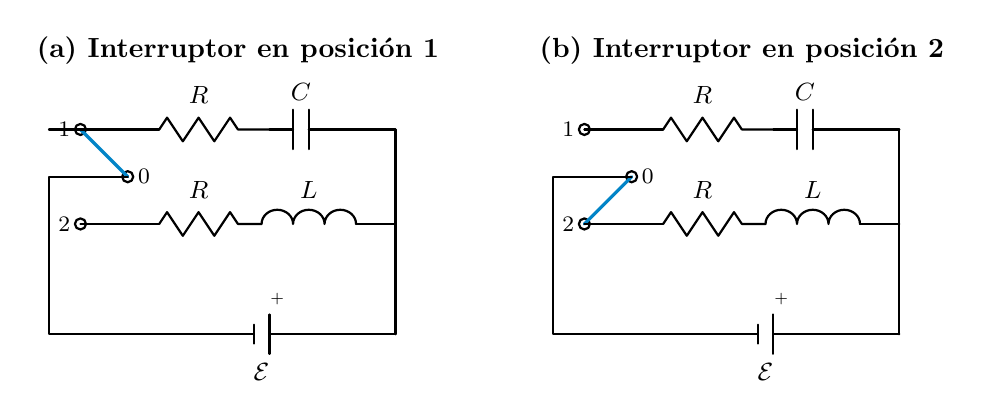
\begin{tikzpicture}[>=Latex, line cap=round, line join=round]

  % Sub-macro o bloque para dibujar el circuito base
  % Posición (a): switch en 1
  \begin{scope}[xshift=0cm]
    \node[above, font=\bfseries] at (2.2, 2.7) {(a) Interruptor en posici\'on 1};

    % Nodos del interruptor: 0 (origen), 1 (rama RC), 2 (rama RL)
    \coordinate (N0) at (0.8, 1.4);
    \coordinate (N1) at (0.2, 2.0);
    \coordinate (N2) at (0.2, 0.8);

    % Círculos de terminales
    \draw[thick] (N0) circle (2pt) node[right, font=\footnotesize] {0};
    \draw[thick] (N1) circle (2pt) node[left, font=\footnotesize] {1};
    \draw[thick] (N2) circle (2pt) node[left, font=\footnotesize] {2};

    % Brazo del interruptor cerrado hacia 1 (rojo o azul)
    \draw[very thick, color=figazul] (N0) -- (N1);

    % Rama superior (conectada a 1): Resistencia R y Capacitor C
    \draw[thick] (N1) -- (-0.2, 2.0) -- (-0.2, 2.0);
    % Conexión hacia la derecha pasando por R y C
    \draw[thick] (0.8, 2.0) -- (1.2, 2.0);
    % Resistor R (zigzag)
    \draw[thick] (1.2, 2.0) -- (1.3, 2.15) -- (1.5, 1.85) -- (1.7, 2.15) -- (1.9, 1.85) -- (2.1, 2.15) -- (2.2, 2.0) -- (2.6, 2.0);
    \node[above, font=\small] at (1.7, 2.2) {$R$};
    % Capacitor C
    \draw[thick] (2.6, 2.0) -- (2.9, 2.0);
    \draw[thick] (2.9, 2.25) -- (2.9, 1.75);
    \draw[thick] (3.1, 2.25) -- (3.1, 1.75);
    \draw[thick] (3.1, 2.0) -- (4.2, 2.0);
    \node[above, font=\small] at (3.0, 2.25) {$C$};

    % Rama inferior (conectada a 2): Resistor R e Inductor L
    \draw[thick] (0.8, 0.8) -- (1.2, 0.8);
    % Resistor R (zigzag)
    \draw[thick] (1.2, 0.8) -- (1.3, 0.95) -- (1.5, 0.65) -- (1.7, 0.95) -- (1.9, 0.65) -- (2.1, 0.95) -- (2.2, 0.8) -- (2.5, 0.8);
    \node[above, font=\small] at (1.7, 1.0) {$R$};
    % Inductor L (bucles/espiras)
    \draw[thick] (2.5, 0.8) arc (180:0:0.2 and 0.18) arc (180:0:0.2 and 0.18) arc (180:0:0.2 and 0.18);
    \draw[thick] (3.7, 0.8) -- (4.2, 0.8);
    \node[above, font=\small] at (3.1, 1.0) {$L$};

    % Conexión vertical derecha que une las ramas
    \draw[thick] (4.2, 2.0) -- (4.2, -0.6);

    % Retorno inferior con Fuente \mathcal{E}
    \draw[thick] (4.2, -0.6) -- (2.6, -0.6);
    % Batería / Fuente \mathcal{E}
    \draw[thick] (2.6, -0.35) -- (2.6, -0.85); % placa larga (+)
    \draw[thick] (2.4, -0.48) -- (2.4, -0.72); % placa corta (-)
    \draw[thick] (2.4, -0.6) -- (-0.2, -0.6) -- (-0.2, 1.4) -- (N0);
    \node[below, font=\small] at (2.5, -0.85) {$\mathcal{E}$};
    \node[above, font=\tiny] at (2.7, -0.35) {$+$};

    % Conexiones del switch hacia ramas
    \draw[thick] (N1) -- (0.8, 2.0);
    \draw[thick] (N2) -- (0.8, 0.8);
  \end{scope}

  % Posición (b): switch en 2
  \begin{scope}[xshift=6.4cm]
    \node[above, font=\bfseries] at (2.2, 2.7) {(b) Interruptor en posici\'on 2};

    % Nodos del interruptor: 0 (origen), 1 (rama RC), 2 (rama RL)
    \coordinate (BN0) at (0.8, 1.4);
    \coordinate (BN1) at (0.2, 2.0);
    \coordinate (BN2) at (0.2, 0.8);

    % Círculos de terminales
    \draw[thick] (BN0) circle (2pt) node[right, font=\footnotesize] {0};
    \draw[thick] (BN1) circle (2pt) node[left, font=\footnotesize] {1};
    \draw[thick] (BN2) circle (2pt) node[left, font=\footnotesize] {2};

    % Brazo del interruptor cerrado hacia 2 (azul)
    \draw[very thick, color=figazul] (BN0) -- (BN2);

    % Rama superior: Resistencia R y Capacitor C
    \draw[thick] (0.8, 2.0) -- (1.2, 2.0);
    \draw[thick] (1.2, 2.0) -- (1.3, 2.15) -- (1.5, 1.85) -- (1.7, 2.15) -- (1.9, 1.85) -- (2.1, 2.15) -- (2.2, 2.0) -- (2.6, 2.0);
    \node[above, font=\small] at (1.7, 2.2) {$R$};
    \draw[thick] (2.6, 2.0) -- (2.9, 2.0);
    \draw[thick] (2.9, 2.25) -- (2.9, 1.75);
    \draw[thick] (3.1, 2.25) -- (3.1, 1.75);
    \draw[thick] (3.1, 2.0) -- (4.2, 2.0);
    \node[above, font=\small] at (3.0, 2.25) {$C$};

    % Rama inferior: Resistor R e Inductor L
    \draw[thick] (0.8, 0.8) -- (1.2, 0.8);
    \draw[thick] (1.2, 0.8) -- (1.3, 0.95) -- (1.5, 0.65) -- (1.7, 0.95) -- (1.9, 0.65) -- (2.1, 0.95) -- (2.2, 0.8) -- (2.5, 0.8);
    \node[above, font=\small] at (1.7, 1.0) {$R$};
    \draw[thick] (2.5, 0.8) arc (180:0:0.2 and 0.18) arc (180:0:0.2 and 0.18) arc (180:0:0.2 and 0.18);
    \draw[thick] (3.7, 0.8) -- (4.2, 0.8);
    \node[above, font=\small] at (3.1, 1.0) {$L$};

    % Conexión vertical derecha
    \draw[thick] (4.2, 2.0) -- (4.2, -0.6);

    % Retorno inferior con Fuente \mathcal{E}
    \draw[thick] (4.2, -0.6) -- (2.6, -0.6);
    \draw[thick] (2.6, -0.35) -- (2.6, -0.85);
    \draw[thick] (2.4, -0.48) -- (2.4, -0.72);
    \draw[thick] (2.4, -0.6) -- (-0.2, -0.6) -- (-0.2, 1.4) -- (BN0);
    \node[below, font=\small] at (2.5, -0.85) {$\mathcal{E}$};
    \node[above, font=\tiny] at (2.7, -0.35) {$+$};

    % Conexiones del switch hacia ramas
    \draw[thick] (BN1) -- (0.8, 2.0);
    \draw[thick] (BN2) -- (0.8, 0.8);
  \end{scope}

\end{tikzpicture}
\end{document}
